\begin{longtable}{|l|l|l|l|l|l|l|}
\hline
Idx & Name & Structure In and Out & Comment & TanTop & DiceMorgan & No. of DescDiff\\
\hline
1 & clopidol & 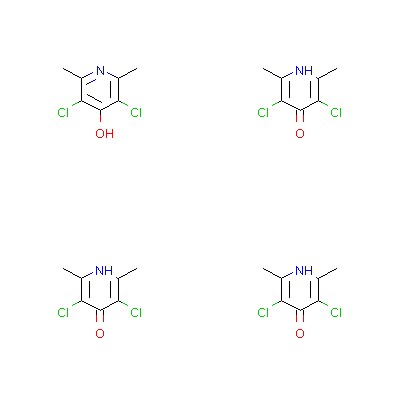
\includegraphics[scale=0.6]{clopidolCA.png} & & [1.0]& [1.0] & [0] \\
\hline
2 & phthalimide & 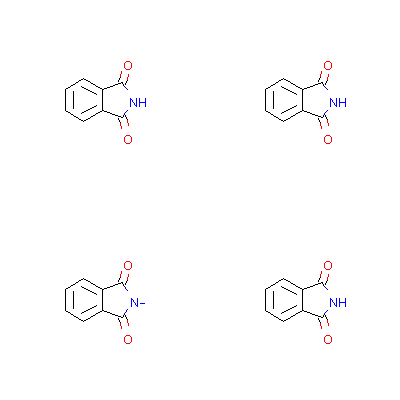
\includegraphics[scale=0.6]{phthalimideCA.png} & & [1.0]& [1.0] & [0] \\
\hline
3 & Viagra & 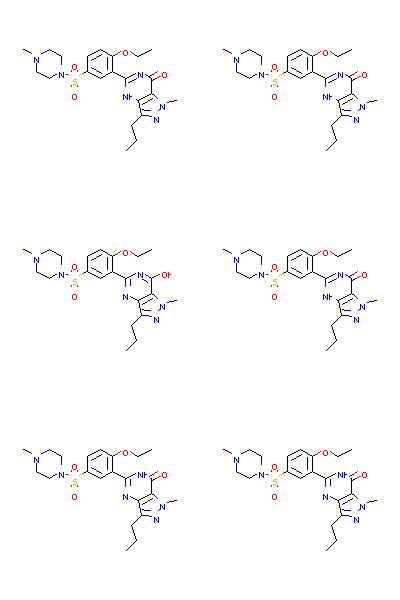
\includegraphics[scale=0.6]{ViagraCA.png} & & [1.0, 1.0, 1.0]& [1.0, 0.91, 0.91] & [1, 21, 21] \\
\hline
4 & quatAmMesomer & 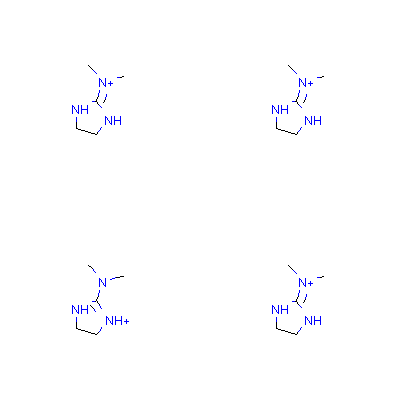
\includegraphics[scale=0.6]{quatAmMesomerCA.png} & & [1.0]& [1.0] & [0] \\
\hline
5 & pyridinol & 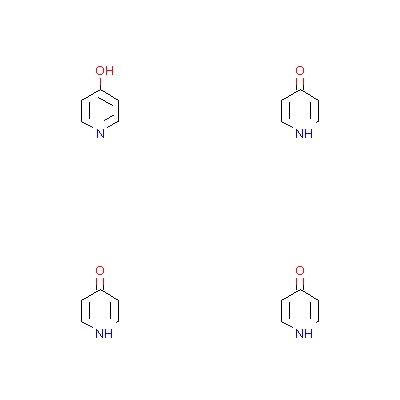
\includegraphics[scale=0.6]{pyridinolCA.png} & & [1.0]& [1.0] & [0] \\
\hline
6 & quatAmMesomer4 & 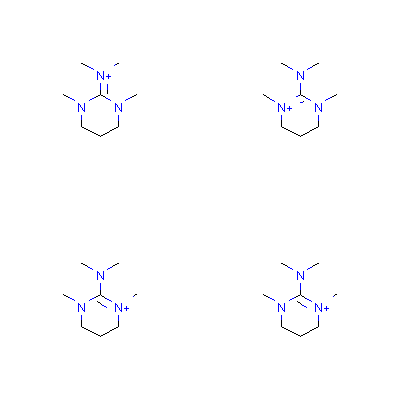
\includegraphics[scale=0.6]{quatAmMesomer4CA.png} & & [1.0]& [1.0] & [1] \\
\hline
7 & azide & 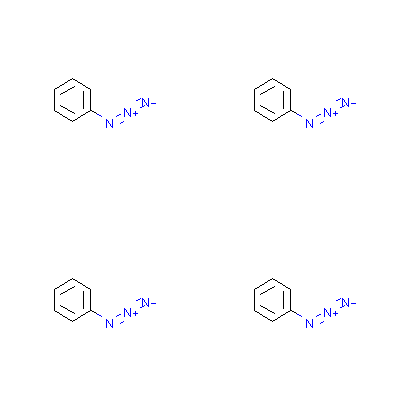
\includegraphics[scale=0.6]{azideCA.png} & & [1.0]& [1.0] & [0] \\
\hline
8 & triazinol & 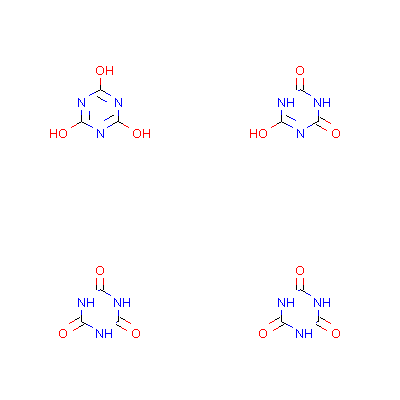
\includegraphics[scale=0.6]{triazinolCA.png} & & [0.58]& [0.54] & [50] \\
\hline
9 & phosphate & 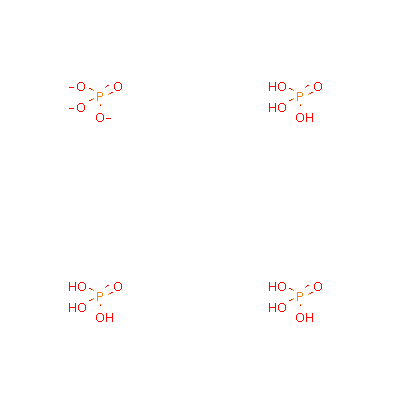
\includegraphics[scale=0.6]{phosphateCA.png} & & [1.0]& [1.0] & [0] \\
\hline
10 & Propenol & 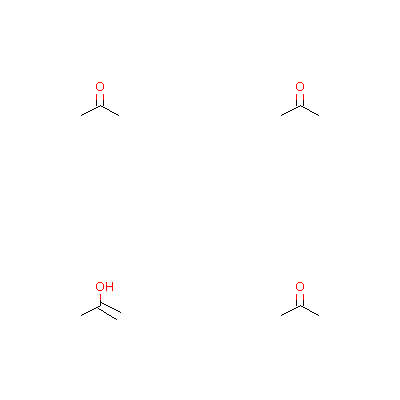
\includegraphics[scale=0.6]{PropenolCA.png} & & [1.0]& [1.0] & [0] \\
\hline
11 & phosphine & 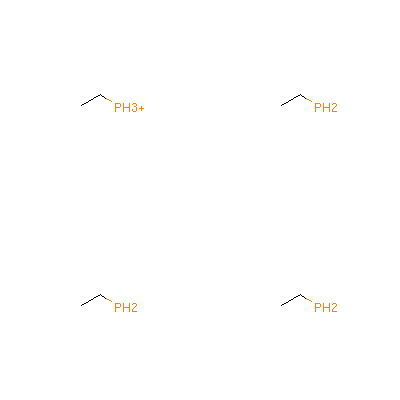
\includegraphics[scale=0.6]{phosphineCA.png} & & [1.0]& [1.0] & [0] \\
\hline
12 & cicletanine & 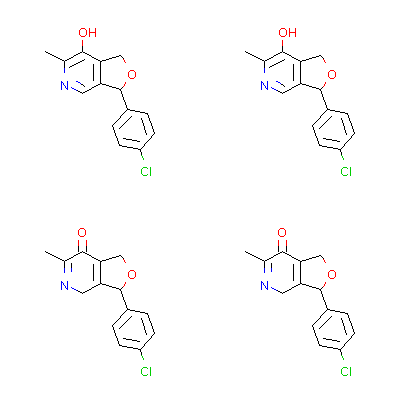
\includegraphics[scale=0.6]{cicletanineCA.png} & & [0.3]& [0.67] & [76] \\
\hline
13 & propaneAcid & 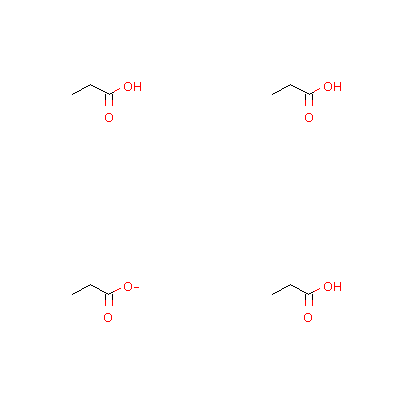
\includegraphics[scale=0.6]{propaneAcidCA.png} & & [1.0]& [1.0] & [0] \\
\hline
14 & imidazole & 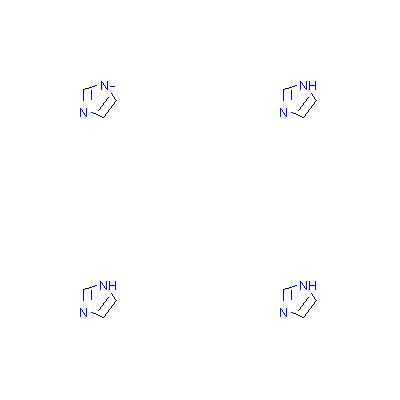
\includegraphics[scale=0.6]{imidazoleCA.png} & & [1.0]& [1.0] & [0] \\
\hline
15 & enamine & 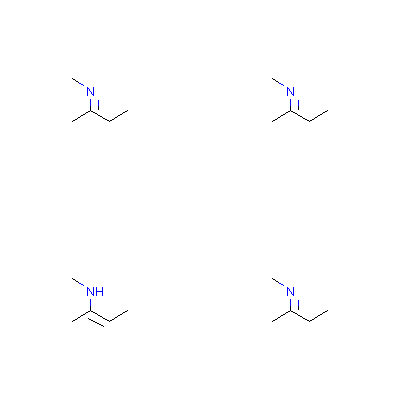
\includegraphics[scale=0.6]{enamineCA.png} & & [1.0]& [1.0] & [0] \\
\hline
16 & sulfoxide & 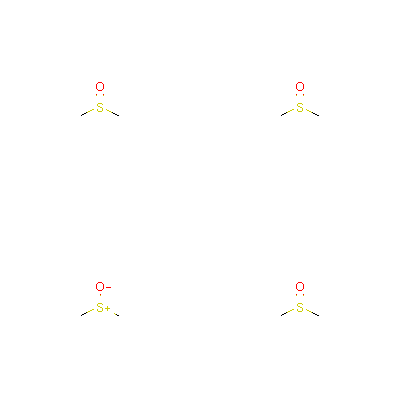
\includegraphics[scale=0.6]{sulfoxideCA.png} & & [1.0]& [1.0] & [0] \\
\hline
17 & sulfonamide & 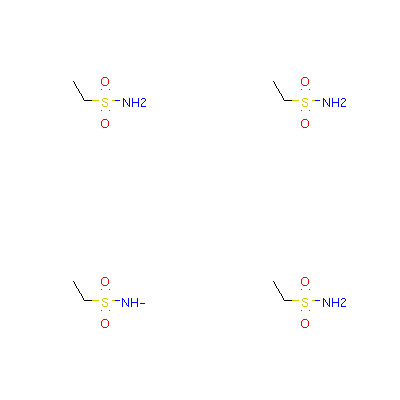
\includegraphics[scale=0.6]{sulfonamideCA.png} & & [1.0]& [1.0] & [0] \\
\hline
18 & tiouracil & 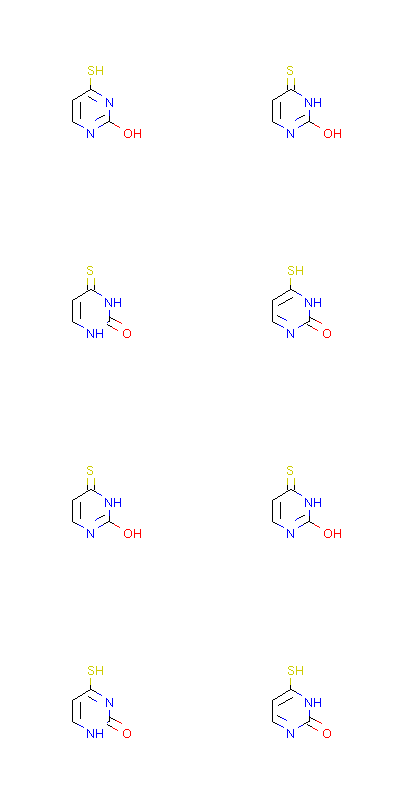
\includegraphics[scale=0.6]{tiouracilCA.png} & & [0.35, 1.0, 0.35, 0.35, 1.0, 0.35]& [0.5, 1.0, 0.5, 0.5, 1.0, 0.5] & [54, 0, 54, 54, 0, 54] \\
\hline
19 & quatAmMesomer2 & 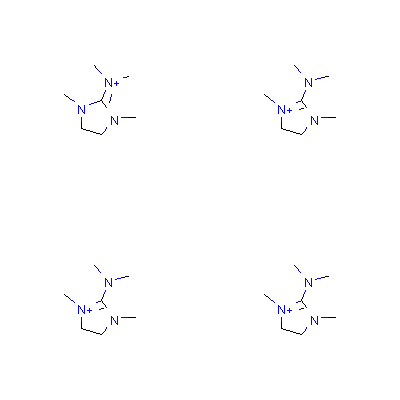
\includegraphics[scale=0.6]{quatAmMesomer2CA.png} & & [1.0]& [1.0] & [0] \\
\hline
20 & nitro & 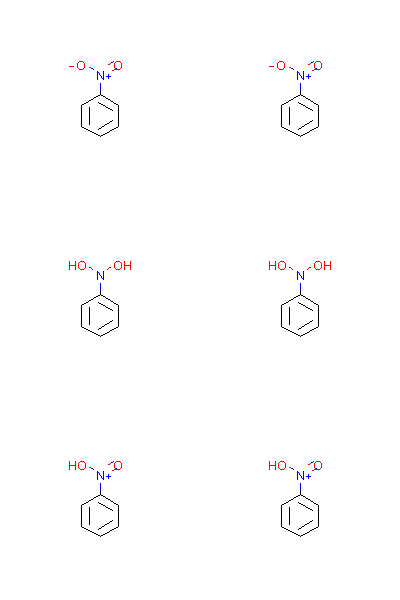
\includegraphics[scale=0.6]{nitroCA.png} & & [0.67, 1.0, 0.67]& [0.56, 0.8, 0.6] & [58, 43, 56] \\
\hline
21 & 107and108and109 & 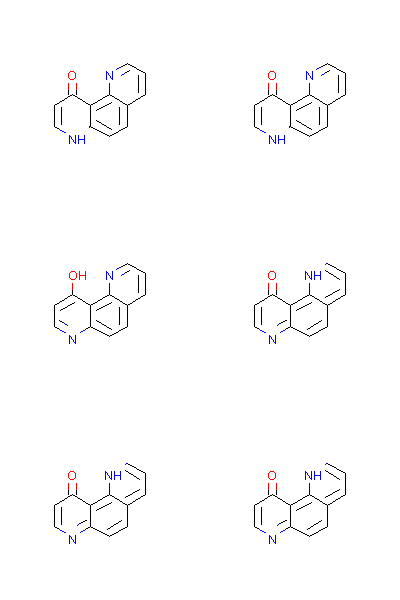
\includegraphics[scale=0.6]{107and108and109CA.png} & & [1.0, 1.0, 1.0]& [0.7, 0.7, 1.0] & [17, 17, 0] \\
\hline
22 & aminopyrimidine & 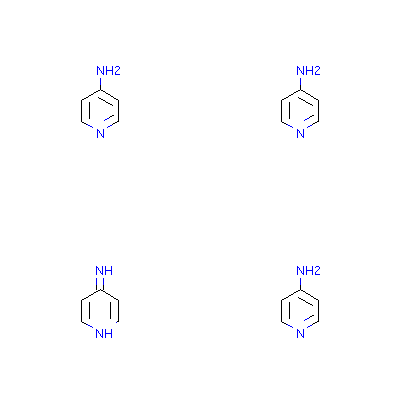
\includegraphics[scale=0.6]{aminopyrimidineCA.png} & & [1.0]& [1.0] & [0] \\
\hline
23 & 105and106 & 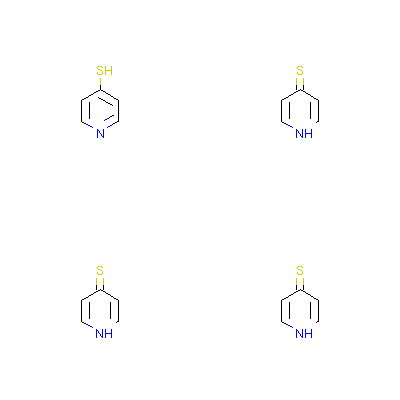
\includegraphics[scale=0.6]{105and106CA.png} & & [1.0]& [1.0] & [0] \\
\hline
24 & Rhodamine & 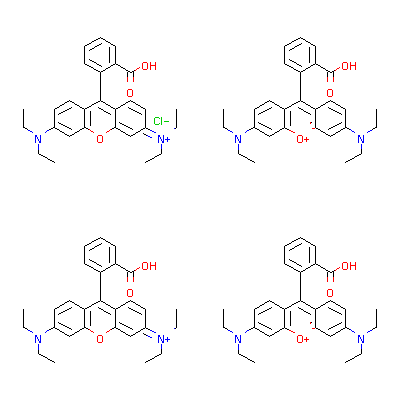
\includegraphics[scale=0.6]{RhodamineCA.png} & & [1.0]& [1.0] & [0] \\
\hline
25 & sulfon & 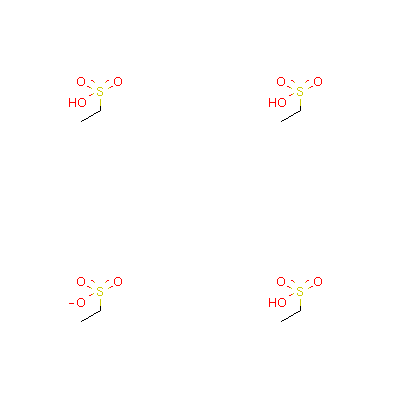
\includegraphics[scale=0.6]{sulfonCA.png} & & [1.0]& [1.0] & [0] \\
\hline
26 & triazine & 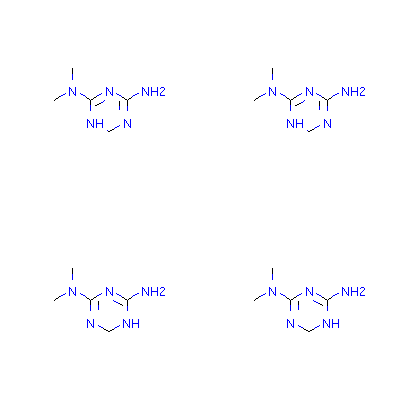
\includegraphics[scale=0.6]{triazineCA.png} & & [0.7]& [0.7] & [21] \\
\hline
27 & tetrazole & 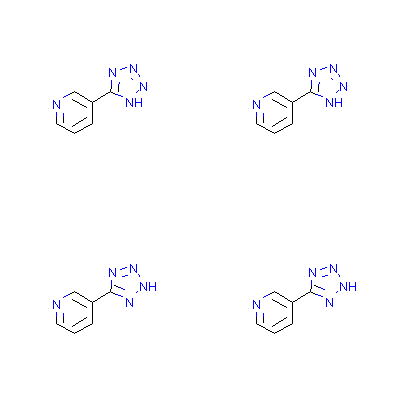
\includegraphics[scale=0.6]{tetrazoleCA.png} & & [1.0]& [0.73] & [22] \\
\hline
28 & phenol & 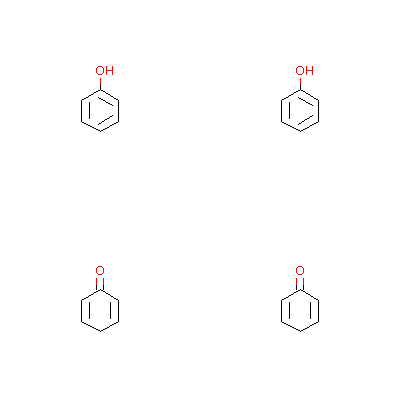
\includegraphics[scale=0.6]{phenolCA.png} & & [0.4]& [0.25] & [68] \\
\hline
29 & phosphor & 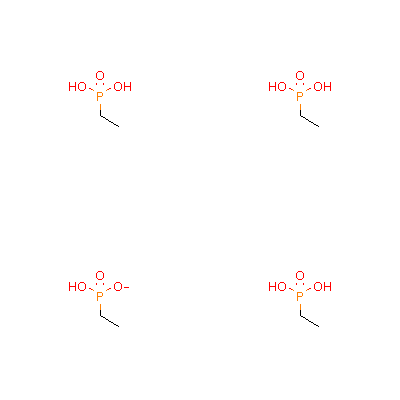
\includegraphics[scale=0.6]{phosphorCA.png} & & [1.0]& [1.0] & [0] \\
\hline
30 & 112and113 & 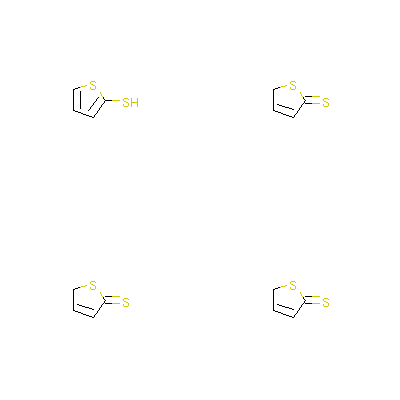
\includegraphics[scale=0.6]{112and113CA.png} & & [1.0]& [1.0] & [0] \\
\hline
31 & NO & 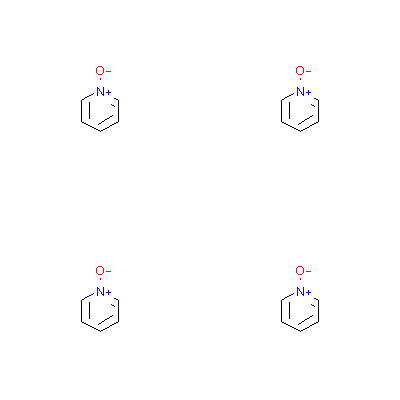
\includegraphics[scale=0.6]{NOCA.png} & & [1.0]& [1.0] & [0] \\
\hline
32 & diazo & 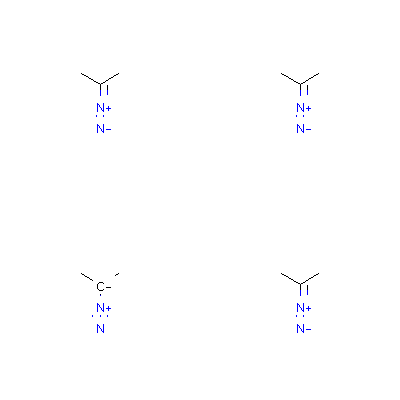
\includegraphics[scale=0.6]{diazoCA.png} & & [1.0]& [1.0] & [0] \\
\hline
33 & benzaldoxime & 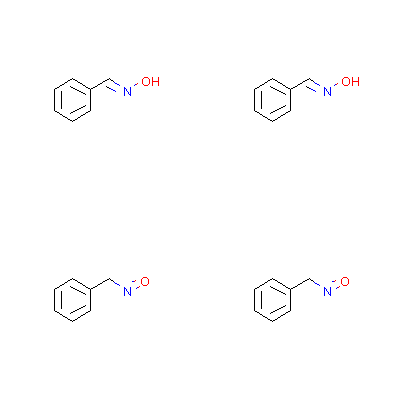
\includegraphics[scale=0.6]{benzaldoximeCA.png} & & [0.57]& [0.58] & [55] \\
\hline
34 & quatAmMesomer3 & 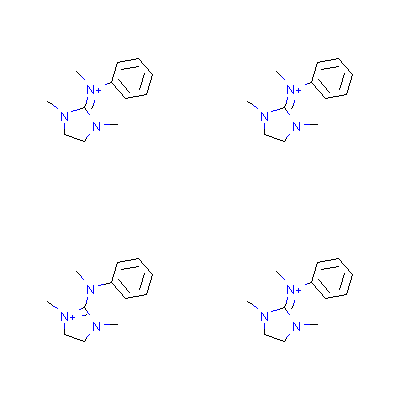
\includegraphics[scale=0.6]{quatAmMesomer3CA.png} & & [1.0]& [1.0] & [0] \\
\hline
35 & NNO & 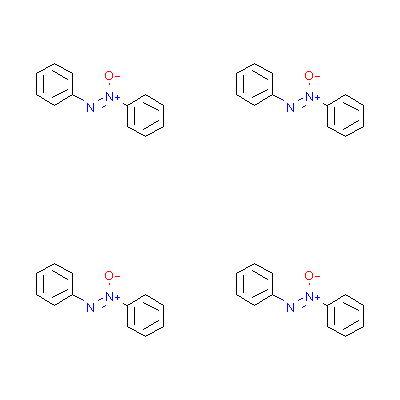
\includegraphics[scale=0.6]{NNOCA.png} & & [1.0]& [1.0] & [0] \\
\hline
36 & amide & 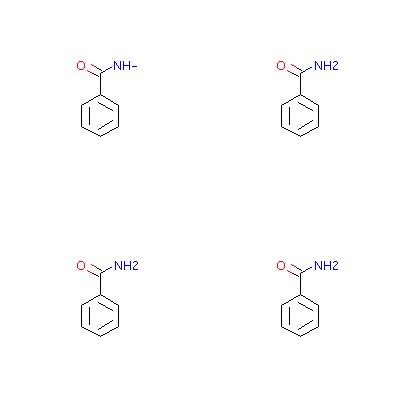
\includegraphics[scale=0.6]{amideCA.png} & & [1.0]& [1.0] & [0] \\
\hline
37 & thiopurine & 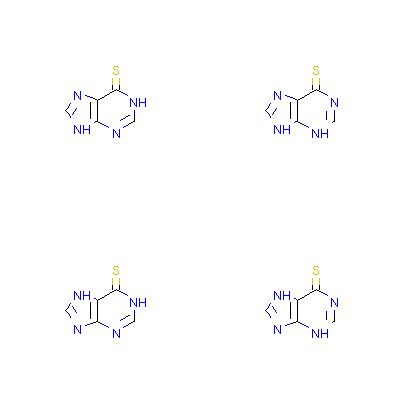
\includegraphics[scale=0.6]{thiopurineCA.png} & & [1.0]& [0.72] & [21] \\
\hline
\end{longtable}